\section{Software}
Softwaren til The Cell Collector udvikles i Matlab. Programmet udvikles af modulær kode, som afgrænser de enkelte funktionaliteter. Blokdiagrammet (figur \ref{fig:bdd_software}) viser hvordan programmet er opdelt i blokke, som afgrænser de enkelte funktionaliteter. 
\subsection{Softwarebeskrivelse}
\begin{figure}[H]
	\centering
	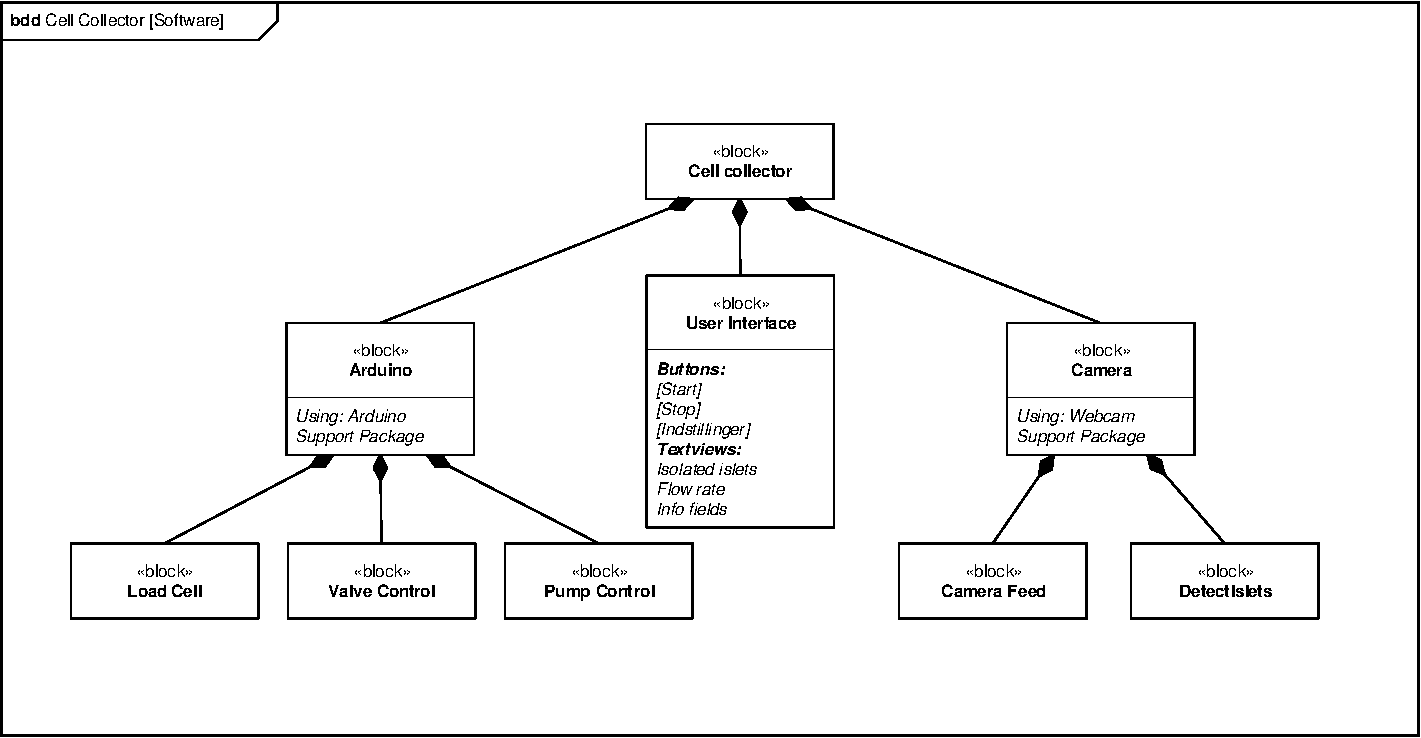
\includegraphics[width=1\textwidth]{billeder/BDD_Software-crop.pdf}
	\caption{BDD - Cell Collector [Software]}
	\label{fig:bdd_software}
\end{figure}


\subsection{Blokbeskrivelser}
\subsubsection{Arduino}
\begin{figure}[H]
	\centering
	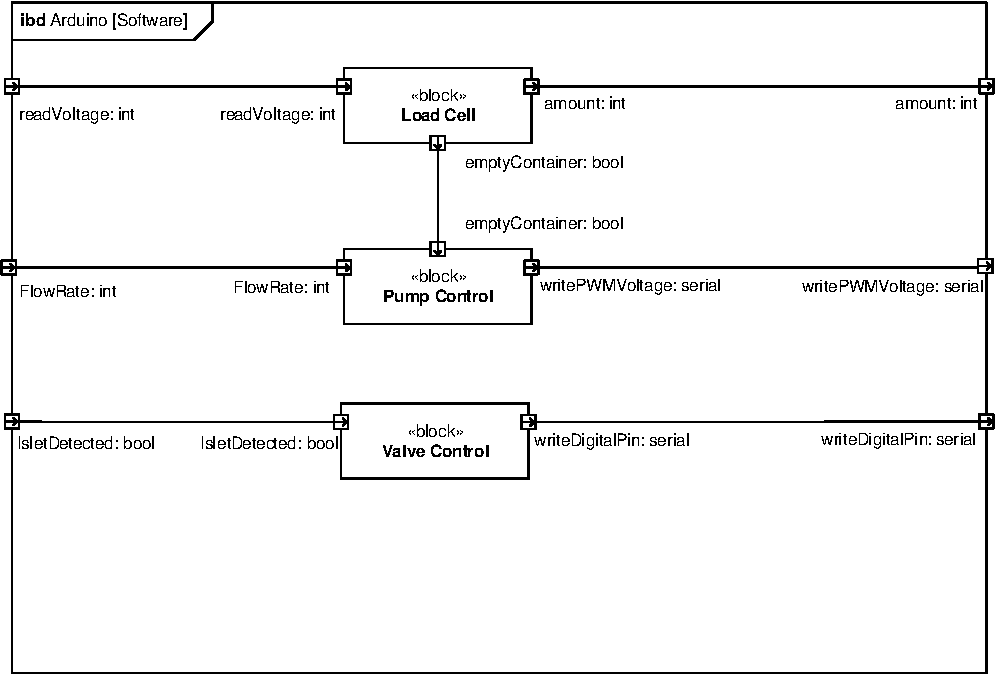
\includegraphics[width=1\textwidth]{billeder/IBD_Software_Arduino-crop.pdf}
	\caption{IBD - Arduino [Software]}
	\label{fig:ibd_software_arduino}
\end{figure}
Beskrivelse om Arduino her
\subsubsection{LoadCell}
LoadCell beskrivelse her
\subsubsection{Pumpe}
\subsubsection{Ventil}


\subsubsection{Kamera}
\begin{figure}[H]
	\centering
	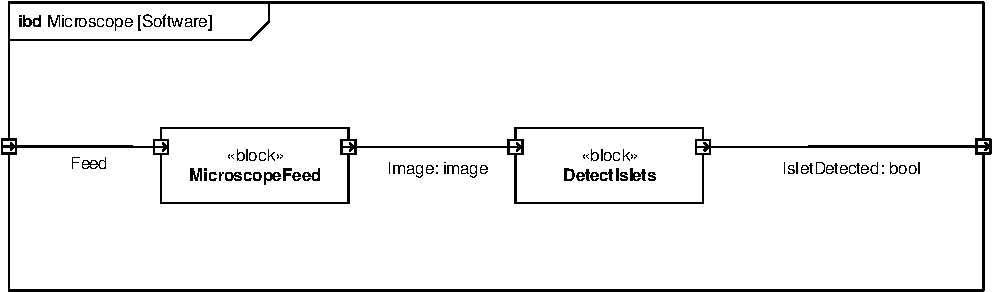
\includegraphics[width=1\textwidth]{billeder/IBD_Software_Kamera-crop.pdf}
	\caption{IBD - Camera [Software]}
	\label{fig:ibd_software_camera}
\end{figure}


\subsection{Funktioner}
\subsection{User Interface}
\subsubsection{Indstillinger}
Mockup
\subsubsection{Callbacks}
Start
Stop
Indstillinger
Indsæt callbacks i form af flowcharts
